\documentclass[border=4pt]{standalone}
\usepackage{fontspec}
\usepackage{amsmath}
\usepackage{unicode-math}
\setmainfont{Latin Modern Roman}
\setmathfont{Latin Modern Math}
\usepackage{pgfplots}
\usepackage{pgfplotstable}
\pgfplotsset{compat=1.18}
\usepackage{tkz-euclide}
\usetikzlibrary{arrows.meta,calc,angles,quotes,patterns,3d,backgrounds}
\definecolor{ink}{HTML}{123428}
\definecolor{asy}{HTML}{475569}
\definecolor{mint}{HTML}{86e0bd}
\tikzset{asym/.style={asy, line width=0.9pt, dash pattern=on 5pt off 3.5pt},
         guide/.style={gray!70, line width=0.6pt, densely dotted},
         dot/.style={circle, inner sep=0pt, minimum size=5pt, draw=white, line width=0.5pt},
         odot/.style={circle, inner sep=0pt, minimum size=5.5pt, fill=white, line width=1pt},
         lab/.style={font=\footnotesize, inner sep=1.5pt, text=ink}}
\begin{document}
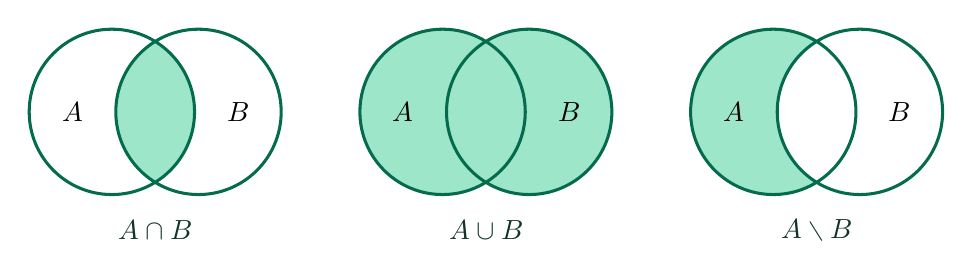
\begin{tikzpicture}[x=1cm, y=1cm]
\begin{scope}\clip (-0.55,0) circle (1.05); \fill[mint!80] (0.55,0) circle (1.05);\end{scope}
\draw[draw={rgb,255:red,4;green,107;blue,77}, line width=1.1pt] (-0.55,0) circle (1.05) (0.55,0) circle (1.05);
\node at (-1.05,0) {$A$}; \node at (1.05,0) {$B$};
\node[text=ink] at (0.0,-1.5) {$A\cap B$};
\fill[mint!80] (3.6500000000000004,0) circle (1.05); \fill[mint!80] (4.75,0) circle (1.05);
\draw[draw={rgb,255:red,4;green,107;blue,77}, line width=1.1pt] (3.6500000000000004,0) circle (1.05) (4.75,0) circle (1.05);
\node at (3.1500000000000004,0) {$A$}; \node at (5.25,0) {$B$};
\node[text=ink] at (4.2,-1.5) {$A\cup B$};
\begin{scope}\fill[mint!80] (7.8500000000000005,0) circle (1.05); \fill[white] (8.950000000000001,0) circle (1.05);\end{scope}
\draw[draw={rgb,255:red,4;green,107;blue,77}, line width=1.1pt] (7.8500000000000005,0) circle (1.05) (8.950000000000001,0) circle (1.05);
\node at (7.3500000000000005,0) {$A$}; \node at (9.450000000000001,0) {$B$};
\node[text=ink] at (8.4,-1.5) {$A\setminus B$};
\end{tikzpicture}
\end{document}
